%%%%%%%%%%%%%%%%%%%%%%%%%%%%%%%%%%%%%%%%%%%%%%%%%%%%%%%%%%%%%%%%%%%%%%%%%%%%%%%
%                       CARGA DE LA CLASE DE DOCUMENTO                        %
%%%%%%%%%%%%%%%%%%%%%%%%%%%%%%%%%%%%%%%%%%%%%%%%%%%%%%%%%%%%%%%%%%%%%%%%%%%%%%%

\documentclass[11pt,spanish,listoffigures,listoftables]{tfgetsinf}

%%%%%%%%%%%%%%%%%%%%%%%%%%%%%%%%%%%%%%%%%%%%%%%%%%%%%%%%%%%%%%%%%%%%%%%%%%%%%%%
%                          CODIFICACIÓN DEL FICHERO                           %
%%%%%%%%%%%%%%%%%%%%%%%%%%%%%%%%%%%%%%%%%%%%%%%%%%%%%%%%%%%%%%%%%%%%%%%%%%%%%%%

\usepackage[utf8]{inputenc} 
\usepackage{babel}
\usepackage{hyperref}
\usepackage{biblatex}
\usepackage{amsmath, amssymb}
\usepackage{graphicx}
\usepackage{booktabs}
\usepackage{listings}
\usepackage{xcolor}
\usepackage{multirow}
\usepackage{subcaption}
\usepackage{tikz}
\usepackage{makecell}
\usetikzlibrary{positioning, calc}

\addbibresource{bib.bib}  % Enlazar el archivo .bib
\addglobalbib{bib.bib}
\hypersetup{ colorlinks=true, linkcolor=black, urlcolor=cyan }

%%%%%%%%%%%%%%%%%%%%%%%%%%%%%%%%%%%%%%%%%%%%%%%%%%%%%%%%%%%%%%%%%%%%%%%%%%%%%%%
%                             OTROS PAQUETES                                  %
%%%%%%%%%%%%%%%%%%%%%%%%%%%%%%%%%%%%%%%%%%%%%%%%%%%%%%%%%%%%%%%%%%%%%%%%%%%%%%%

%%%%%%%%%%%%%%%%%%%%%%%%%%%%%%%%%%%%%%%%%%%%%%%%%%%%%%%%%%%%%%%%%%%%%%%%%%%%%%%
%                         DATOS DEL TRABAJO                                   %
%%%%%%%%%%%%%%%%%%%%%%%%%%%%%%%%%%%%%%%%%%%%%%%%%%%%%%%%%%%%%%%%%%%%%%%%%%%%%%%

\title{Clasificación automática de artrosis en rodillas mediante redes neuronales convolucionales}
\author{Hernández Martínez, Carlos}
\tutor{Juan Ciscar, Alfonso}
\curs{2024-2025}

%%%%%%%%%%%%%%%%%%%%%%%%%%%%%%%%%%%%%%%%%%%%%%%%%%%%%%%%%%%%%%%%%%%%%%%%%%%%%%%
%            PALABRAS CLAVE Y RESÚMENES (en tres idiomas)                     %
%%%%%%%%%%%%%%%%%%%%%%%%%%%%%%%%%%%%%%%%%%%%%%%%%%%%%%%%%%%%%%%%%%%%%%%%%%%%%%%

\keywords{Palabras clave en catalán} % catalán
         {Palabras clave en español} % español
         {Keywords in English}       % inglés

% Añade esto en el preámbulo (antes de \begin{document})
\setcounter{tocdepth}{1} % Muestra solo capítulos y secciones en el índice
\begin{document}

%%%%%%%%%%%%%%%%%%%%%%%%%%%%%%%%%%%%%%%%%%%%%%%%%%%%%%%%%%%%%%%%%%%%%%%%%%%%%%%
%                             RESÚMENES                                       %
%%%%%%%%%%%%%%%%%%%%%%%%%%%%%%%%%%%%%%%%%%%%%%%%%%%%%%%%%%%%%%%%%%%%%%%%%%%%%%%

\begin{abstract}

El presente Trabajo de Fin de Grado (TFG) aborda el desarrollo de un sistema de clasificación automática de artrosis en rodillas mediante redes neuronales convolucionales (CNN), una técnica avanzada de aprendizaje profundo (Deep Learning). La artrosis es una de las enfermedades musculoesqueléticas más prevalentes a nivel mundial, caracterizada por la degeneración del cartílago articular y que afecta principalmente a adultos mayores. Sin embargo, su diagnóstico sigue siendo un proceso subjetivo que depende en gran medida de la interpretación visual de imágenes médicas por parte de especialistas.

Para enfrentar esta problemática, se ha implementado un modelo basado en redes neuronales convolucionales entrenado con el dataset OAI (Osteoarthritis Initiative), que contiene radiografías de rodillas etiquetadas según la escala Kellgren-Lawrence (KL), un estándar clínico para evaluar la severidad de la enfermedad. El sistema propuesto se ha diseñado utilizando distintas arquitecturas de redes, incluyendo modelos desde cero y redes preentrenadas (Transfer Learning) adaptadas para esta tarea.

El desarrollo del sistema ha seguido un enfoque incremental, evaluando el desempeño de modelos simples y progresivamente complejos, comparando métricas de precisión, F1-score y error absoluto medio (MAE) en la clasificación de imágenes. Adicionalmente, se ha explorado la capacidad de generalización del modelo aplicándolo a un conjunto externo de imágenes de radiografías de gatos, simulando una transferencia de conocimiento hacia otro dominio anatómico.

Los resultados obtenidos muestran que las redes convolucionales profundas, especialmente aquellas ajustadas mediante aprendizaje por transferencia, ofrecen un rendimiento superior en la clasificación del grado de artrosis, alcanzando niveles de precisión comparables a los de estudios previos en la literatura. No obstante, también se identificaron desafíos relacionados con el desbalance de clases en el dataset y la necesidad de técnicas avanzadas de interpretación de modelos, como Grad-CAM.

En conclusión, este TFG demuestra la viabilidad del uso de redes neuronales convolucionales para la clasificación automática de artrosis en rodillas, destacando el potencial de estas técnicas para apoyar la labor diagnóstica de los profesionales médicos y abriendo la posibilidad de extender el sistema a otros dominios, como la artrosis en animales.

\end{abstract}



\begin{abstract}[english]
    
This Final Degree Project (TFG) addresses the development of an automatic classification system for knee osteoarthritis using Convolutional Neural Networks (CNNs), an advanced deep learning technique. Osteoarthritis is one of the most prevalent musculoskeletal diseases worldwide, characterized by the degeneration of articular cartilage, primarily affecting older adults. However, its diagnosis remains a subjective process, heavily dependent on the visual interpretation of medical images by specialists.
    
To tackle this problem, a model based on convolutional neural networks was implemented, trained with the OAI (Osteoarthritis Initiative) dataset, which contains knee radiographs labeled according to the Kellgren-Lawrence (KL) scale, a clinical standard for assessing disease severity. The proposed system was designed using various network architectures, including models built from scratch and pre-trained networks (Transfer Learning) adapted for this task.
    
The system development followed an incremental approach, evaluating the performance of simple and progressively complex models, comparing metrics such as accuracy, F1-score, and Mean Absolute Error (MAE) in image classification. Additionally, the model's generalization capability was explored by applying it to an external set of cat knee radiographs, simulating knowledge transfer to another anatomical domain.
    
The results obtained show that deep convolutional networks, especially those adjusted through transfer learning, offer superior performance in classifying the severity of osteoarthritis, achieving precision levels comparable to previous studies in the literature. However, challenges related to class imbalance in the dataset and the need for advanced model interpretation techniques, such as Grad-CAM, were also identified.
    
In conclusion, this TFG demonstrates the feasibility of using convolutional neural networks for the automatic classification of knee osteoarthritis, highlighting the potential of these techniques to support the diagnostic work of medical professionals and opening the possibility of extending the system to other domains, such as osteoarthritis in animals.
    
\end{abstract}

\mainmatter

%%%%%%%%%%%%%%%%%%%%%%%%%%%%%%%%%%%%%%%%%%%%%%%%%%%%%%%%%%%%%%%%%%%%%%%%%%%%%%%
%                              CAPÍTULO 1                                     %
%                                    INTRO                                     %
%%%%%%%%%%%%%%%%%%%%%%%%%%%%%%%%%%%%%%%%%%%%%%%%%%%%%%%%%%%%%%%%%%%%%%%%%%%%%%%

\chapter{Introducción}  % ~5 páginas

\section{Motivación}     % 1.1
La artritis es una de las enfermedades musculoesqueléticas más prevalentes a nivel mundial y una de las principales causas de discapacidad en adultos mayores. Su diagnóstico y seguimiento se basa tradicionalmente en la evaluación clínica y en la interpretación de imágenes médicas, como radiografías, resonancias magnéticas y tomografías computarizadas. Sin embargo, este proceso suele depender en gran medida de la experiencia del profesional médico, lo que puede generar variabilidad en los diagnósticos y retrasos en la detección temprana de la enfermedad.

En los últimos años, los avances en inteligencia artificial, y en particular en el aprendizaje profundo, han demostrado un gran potencial para mejorar la precisión y la eficiencia en el análisis de imágenes médicas. Las redes neuronales convolucionales (CNN) han sido ampliamente utilizadas en el campo de la visión por computadora para tareas como la detección de patologías en radiografías, la segmentación de tejidos en resonancias magnéticas y la clasificación de niveles de severidad en enfermedades degenerativas.

Este Trabajo de Fin de Grado (TFG) se motiva por la necesidad de desarrollar métodos automáticos y robustos para el análisis de la artritis mediante el uso de técnicas de aprendizaje profundo. En particular, se busca explorar el uso de redes neuronales para la clasificación de imágenes médicas, utilizando bases de datos estandarizadas como \textit{Mendeley dataset} \cite{chen2018knee}. La aplicación de estos modelos podría no solo optimizar el proceso de diagnóstico, sino también contribuir al desarrollo de herramientas de soporte a la decisión clínica, facilitando una intervención más temprana y personalizada para los pacientes.

La relevancia de este estudio radica en su potencial impacto en la práctica clínica. Un sistema basado en inteligencia artificial podría reducir la carga de trabajo de los especialistas, mejorar la objetividad del diagnóstico y ofrecer segundas opiniones automáticas que complementen la evaluación médica tradicional. Además, el desarrollo de estas tecnologías en el ámbito de la artritis podría sentar un precedente para su aplicación en otras enfermedades musculoesqueléticas, ampliando el alcance del aprendizaje profundo en el campo de la salud.

Además, se plantea la posibilidad de realizar \textit{transfer learning} utilizando modelos preentrenados en artritis humana para aplicarlos en el diagnóstico de artritis en gatos. Esta adaptación podría beneficiar la práctica veterinaria, proporcionando herramientas automatizadas para la evaluación de la enfermedad en animales y mejorando la precisión en su diagnóstico.

En este contexto, el presente trabajo busca contribuir al avance del uso de inteligencia artificial en la detección y análisis de la artritis, evaluando diferentes enfoques de redes neuronales y analizando su rendimiento en la clasificación de imágenes médicas. La motivación principal es demostrar la viabilidad y efectividad de estos modelos en un problema biomédico concreto, promoviendo la integración de tecnologías emergentes en el ámbito de la salud.



\section{Objetivos del TFG}

El presente Trabajo de Fin de Grado (TFG) tiene como objetivo desarrollar un sistema de clasificación automática de artrosis en rodillas mediante redes neuronales convolucionales (CNN). Este objetivo se justifica en la necesidad de mejorar la precisión y eficiencia del diagnóstico de la artrosis, una enfermedad que afecta a millones de personas en todo el mundo, y que actualmente depende en gran medida de la interpretación subjetiva de imágenes radiográficas por parte de especialistas.

Para alcanzar este objetivo general, se plantean los siguientes objetivos específicos:

\begin{itemize}
\item \textbf{Desarrollar un modelo de clasificación automática de artrosis en rodillas} utilizando redes neuronales convolucionales (CNN). Este modelo será entrenado y evaluado sobre el conjunto de datos OAI (Osteoarthritis Initiative), uno de los recursos más utilizados en la literatura para el estudio de la artrosis de rodilla. El desarrollo incluirá una fase de diseño, implementación y ajuste de hiperparámetros para maximizar el rendimiento.

```
\item \textbf{Evaluar la capacidad de transferencia del modelo a otro dominio anatómico}, aplicando técnicas de aprendizaje por transferencia (Transfer Learning). En concreto, se analizará cómo el modelo, entrenado en imágenes de rodillas humanas, puede adaptarse a la clasificación de artrosis en radiografías de gatos. Esto permitirá estudiar el impacto del cambio de dominio en el rendimiento del modelo y su capacidad de generalización.

\item \textbf{Analizar el rendimiento del modelo propuesto}, evaluando su precisión, sensibilidad, especificidad, F1-score y MAE. Además, se identificarán las limitaciones del modelo y las fuentes de error, proponiendo posibles mejoras mediante técnicas avanzadas de aprendizaje profundo, como la optimización de arquitecturas, ajuste fino (fine-tuning) y visualización interpretativa con Grad-CAM.
```

\end{itemize}

Con estos objetivos, el presente TFG busca no solo desarrollar un sistema eficiente para la clasificación de artrosis, sino también aportar un análisis crítico de su rendimiento y explorar estrategias para su optimización.


\section{Estructura del documento}  % 1.3
% Describe la organización de los capítulos y secciones

%%%%%%%%%%%%%%%%%%%%%%%%%%%%%%%%%%%%%%%%%%%%%%%%%%%%%%%%%%%%%%%%%%%%%%%%%%%%%%%
%                              CAPÍTULO 2                                     %
%                                PRELIMINARES (STANDBY)                       %
%%%%%%%%%%%%%%%%%%%%%%%%%%%%%%%%%%%%%%%%%%%%%%%%%%%%%%%%%%%%%%%%%%%%%%%%%%%%%%%

\chapter{Preliminares}  % ~15 páginas
\section{Aprendizaje automático}


El \textbf{aprendizaje automático} (ML) es una rama de la inteligencia artificial que se enfoca en que las máquinas mejoren 
su desempeño en una tarea determinada a partir de la experiencia. Un sistema \textit{“aprende”} cuando su desempeño en una tarea, 
medido por una métrica, mejora con la experiencia adquirida. En términos prácticos, esto implica diseñar algoritmos capaces de 
\textit{generalizar} patrones a partir de datos, de forma que puedan hacer predicciones o tomar decisiones sobre datos no vistos 
previamente. En aprendizaje automático se suelen representar los datos con un conjunto de \textit{características} (features) relevantes, y el algoritmo 
construye un modelo matemático que relaciona estas características con las salidas esperadas. Un objetivo central es lograr un buen 
equilibrio entre \textit{ajuste} a los datos de entrenamiento y \textit{capacidad de generalización} a nuevos datos, evitando problemas 
como el \textit{sobreajuste} (overfitting). La Figura~\ref{fig:overfitting} ilustra de forma visual las diferencias entre 
subajuste, buen ajuste y sobreajuste en un modelo supervisado, conceptos fundamentales para entender el rendimiento de los modelos de aprendizaje automático.

\begin{figure}[ht]
    \centering
    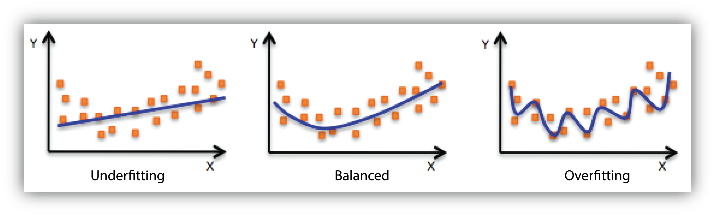
\includegraphics[width=0.7\textwidth]{under-overfitting.png}
    \caption{Ejemplo ilustrativo de subajuste, buen ajuste y sobreajuste en un modelo supervisado. Adaptado de \cite{awsOverfitting}.}
    \label{fig:overfitting}
\end{figure}

Existen varias categorías principales de aprendizaje automático, diferenciadas por la forma en que el algoritmo recibe la información 
y el tipo de tarea a resolver:
\begin{itemize}
    \item \textbf{Aprendizaje supervisado}: El algoritmo recibe ejemplos de entrada y su correspondiente salida deseada (etiquetas). 
    El objetivo es aprender una función que mapee las entradas a las salidas correctas. Son tareas típicas la \textit{clasificación} 
    (p. ej., dado un conjunto de características de un paciente, predecir que enfermedad tiene: salida categórica) y la 
    \textit{regresión} (p. ej., dada las características de una casa predecir su precio). El rendimiento se evalúa comúnmente con funciones
    que relacionan la predicción del modelo con el valor real (p. ej. error cuadrático en regressión o entropía cruzada en clasificación).

    \item \textbf{Aprendizaje no supervisado}: El algoritmo recibe datos de entrada sin etiquetas, y debe descubrir estructura oculta en 
    ellos. Incluye tareas como la \textit{clustering} (agrupamiento de datos por similitud) o la \textit{reducción de dimensionalidad} 
    (encontrar representaciones más compactas de los datos). Un claro ejemplo de aprendizaje no supervisado consiste en la agrupación de
    correos en distintos tipos.
    
    \item \textbf{Aprendizaje por refuerzo}: El algoritmo (un \textit{agente}) aprende a través de la interacción con un entorno, 
    recibiendo recompensas o penalizaciones según sus acciones. El agente debe descubrir una política de acciones que maximice la 
    recompensa acumulada. Este paradigma es común en robótica y juegos, donde no se proporcionan ejemplos de solución directa sino una 
    señal de calidad de cada acción.
    
\end{itemize}

En el ámbito médico se utiliza comunmente el \textbf{aprendizaje supervidado}. El proceso típico de esta tarea consiste en entrenar
un modelo ajustando sus parámetros para minimizar una función de error o \textit{función de pérdida} (loss function) que mide el error 
de las predicciones del modelo sobre los datos de entrenamiento. El procedimiento de optimización más utilizado es el 
\textit{descenso de gradiente} y sus variantes, como el descenso de gradiente estocástico, que permite procesar los datos por lotes. 
En cada iteración, se calcula la gradiente del error respecto a los parámetros del modelo, y se ajustan los parámetros en la dirección 
opuesta a dicha gradiente para reducir el error. Este ciclo se repite múltiples veces (\textit{épocas}) 
hasta converger a un mínimo local del error.

La Figura~\ref{fig:gd_flow} muestra esquemáticamente el flujo de este proceso, donde la posicion inicial tiene el error máximo y en cada
iteración se va reduciendo el error (como una pelota que rueda por una pendiente). A continuación, el Algoritmo~\ref{alg:gd-train} detalla 
los pasos fundamentales que se siguen durante el entrenamiento de un modelo mediante esta técnica.

\begin{figure}[ht]
    \centering
    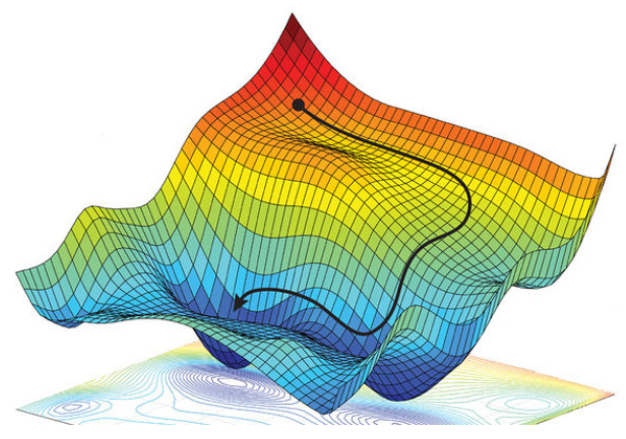
\includegraphics[width=0.8\textwidth]{descenso_gradiente.png}
    \caption{Flujo de entrenamiento de un modelo supervisado mediante descenso de gradiente. Adaptado de \cite{logongasBackprop}.}
    \label{fig:gd_flow}
\end{figure}

\begin{algorithmic}
    \label{alg:gd-train}
    \REQUIRE Conjunto de entrenamiento ${(x_i, y_i)}_{i=1}^N$, tasa de aprendizaje $\eta$ función de error $\mathcal{L}$
    \STATE Inicializar parámetros del modelo $\theta$ (p. ej. aleatoriamente)
    \FOR{numero de épocas}
        \FOR{cada $(x_i, y_i)$ en ${(x_i, y_i)}_{i=1}^N$}
            \STATE calcular predicción $\hat{y}_i = f_\theta(x_i)$
            \STATE calcular pérdida $L = \mathcal{L}(\hat{y}_i, y_i)$ \COMMENT{ej.: error cuadrático, entropía cruzada, etc.}
            \STATE calcular gradiente $g = \nabla_{\theta} L$
            \STATE actualizar parámetros: $\theta := \theta - \eta \cdot g$
        \ENDFOR
    \ENDFOR
\end{algorithmic}

Tras el entrenamiento, es fundamental evaluar el modelo con datos independientes (conjunto de \textit{prueba}) para estimar su capacidad de generalización. 
Además, suelen emplearse técnicas como \textit{validación cruzada} y conjuntos de \textit{validación} para ajustar hiperparámetros (parámetros del algoritmo 
que no se aprenden directamente, como la profundidad de un árbol de decisión o la tasa de aprendizaje $\eta$). Un buen enfoque de validación ayuda a prevenir 
el sobreajuste y a seleccionar modelos más robustos.

Existen algoritmos clásicos de ML como los \textit{árboles de decisión}, \textit{máquinas de vector soporte} (SVM), \textit{vecinos más cercanos} (k-NN), entre otros,
cada uno con sus supuestos y ámbitos de aplicación. Por ejemplo, las SVM buscan hiperplanos que separen clases maximizando el margen, mientras que los árboles de 
decisión realizan particiones recursivas del espacio de características para homogeneizar las etiquetas en los nodos hoja. La elección del algoritmo adecuado depende 
de la naturaleza de los datos y del problema a resolver, no existiendo un modelo único que sea óptimo para todas las tareas.

En resumen, el aprendizaje automático proporciona las bases para construir modelos que extraen conocimiento de los datos. Estos conceptos preliminares resultan 
imprescindibles para entender técnicas más avanzadas como las redes neuronales profundas y su aplicación en tareas de visión por computador y medicina, que se 
abordan en secciones posteriores.

\section{Redes Neuronales}\label{sec:nn} 

Las \textbf{redes neuronales artificiales} (RNA) constituyen una familia de modelos de aprendizaje automático inspirados vagamente en el cerebro humano. 
La unidad básica de una RNA es la \textit{neurona artificial}, un elemento que realiza una operación sencilla: calcula una combinación lineal de sus entradas y 
le aplica una función no lineal llamada \textit{función de activación}. Matemáticamente, si una neurona recibe como entradas $x_1, x_2, \dots, x_n$ con pesos 
sinápticos $w_1, w_2, \dots, w_n$ y tiene un sesgo $b$, produce una salida $y = \sigma(w_1 x_1 + w_2 x_2 + \cdots + w_n x_n + b)$, donde $\sigma(\cdot)$ podría ser, 
por ejemplo, una función sigmoide, tangente hiperbólica o ReLU (Unidad Lineal Rectificada). Las primeras RNA, como el \textit{Perceptrón} de Rosenblatt,  tenían una 
sola capa de neuronas (una capa de entrada proyectada directamente a una capa de salida) y podían aprender a clasificar datos que fueran linealmente separables. 
Sin embargo, se demostró que una sola neurona (o capa lineal) tiene limitaciones significativas en su capacidad de representación.

La potencia de las redes neuronales radica en su capacidad para formar \textbf{arquitecturas multicapa}, también conocidas como \textit{redes neuronales de múltiples capas} 
o \textit{perceptrones multicapa} (MLP). Estas redes están organizadas en capas: una capa de entrada (los datos originales), una o varias capas \textit{ocultas} que 
realizan transformaciones intermedias mediante neuronas con sus pesos, y una capa de salida que produce la predicción final. Al agregar capas ocultas con funciones de 
activación no lineales, las redes adquieren la habilidad de aproximar relaciones no lineales arbitrariamente complejas entre la entrada y la salida. En la imagen
\ref{fig:neural_network} se observa un ejemplo de una red neuronal profunda, donde cada círculo representa una neurona y las líneas indican las conexiones entre ellas.

\begin{figure}[htbp]
    \centering
    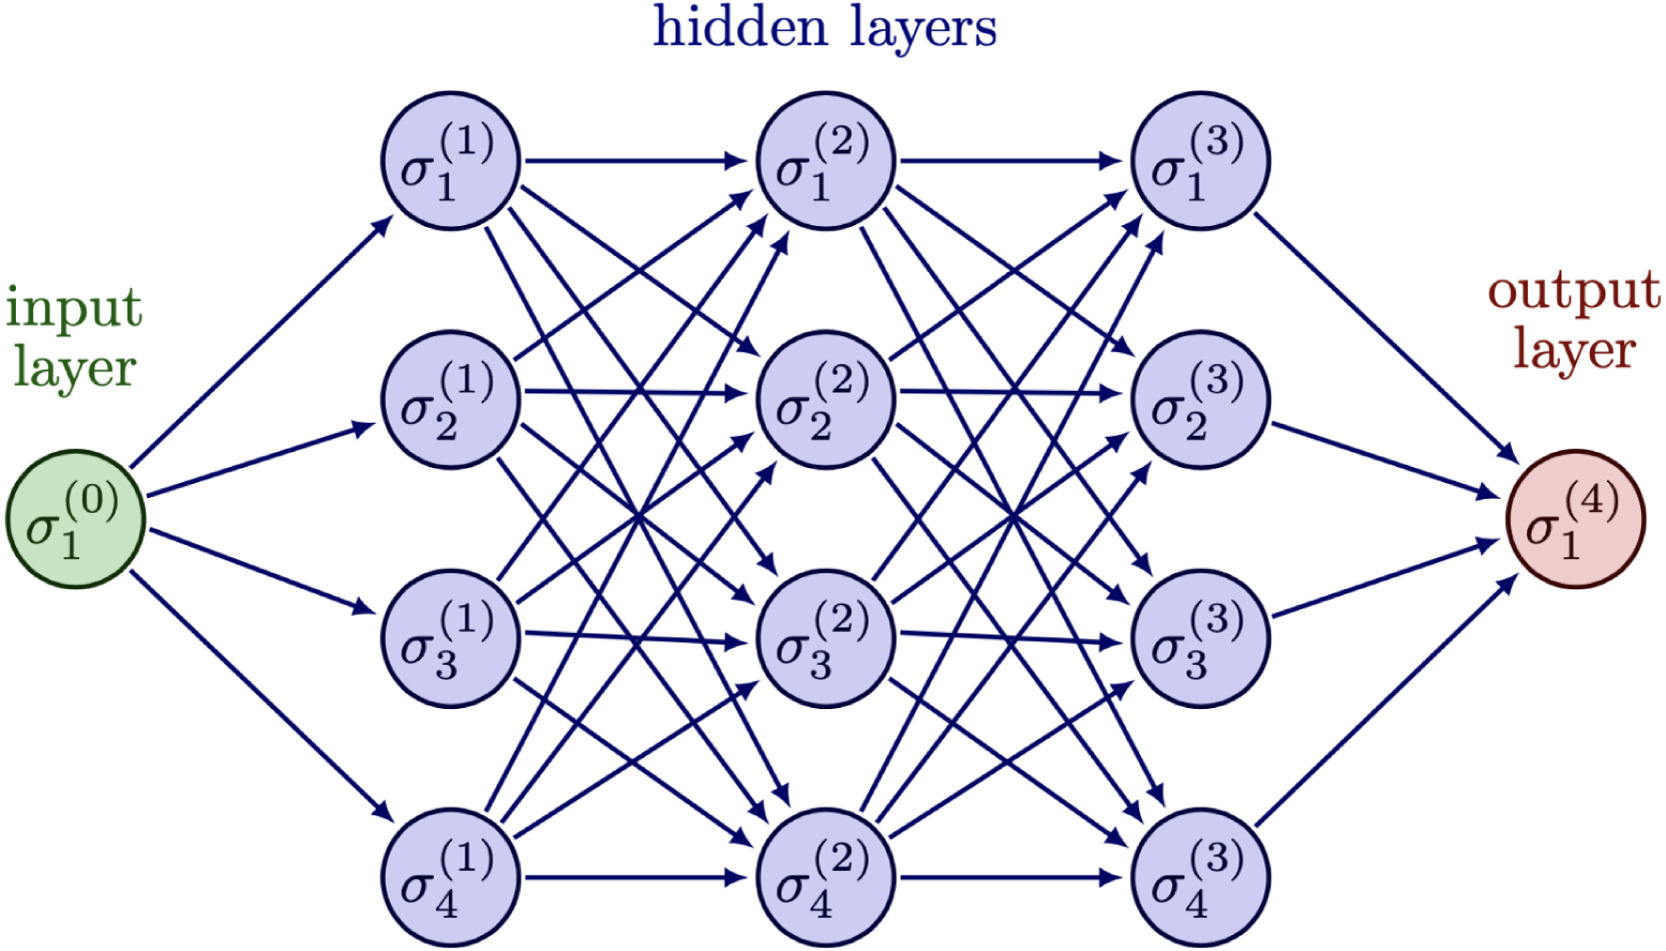
\includegraphics[width=0.5\textwidth]{neural_network.jpg}
    \caption{Ejemplo de una red neuronal profunda \cite{neural_network}}
    \label{fig:neural_network}
\end{figure}


El entrenamiento de una red neuronal multicapa se realiza típicamente mediante el algoritmo de \textit{retropropagación del error} (backpropagation) combinado con 
descenso de gradiente. En esencia, el procedimiento es: se calculan las salidas de la red para una entrada dada (\textit{fase forward}), se mide el error cometido 
comparando con la salida deseada mediante una función de coste (por ejemplo, la entropía cruzada para clasificación), y luego se propaga ese error hacia atrás a 
través de la red (\textit{fase backward}) calculando las derivadas parciales del error con respecto a cada peso utilizando la regla de la cadena. Estas derivadas 
indican cómo ajustar cada peso para reducir el error, y se aplican las actualizaciones de los pesos en consecuencia. Gracias a la retropropagación, las redes neuronales 
pueden entrenarse eficientemente incluso con muchas capas, ajustando millones de parámetros para adaptarse a complejos conjuntos de datos. Este avance fue crucial para 
el renacimiento de las redes neuronales en la década de 1980, tras un período de estancamiento parcial debido a las limitaciones de los perceptrones simples destacadas 
por Minsky y Papert en 1969 (quienes señalaron, por ejemplo, que un perceptrón no podía aprender la función XOR). El trabajo de Rumelhart, Hinton y Williams (1986) 
introdujo formalmente la retropropagación, mostrando que las redes de múltiples capas podían aprender características jerárquicas y superar esas limitaciones previas.

A medida que se dispuso de más datos y mayor potencia de cómputo, especialmente con la llegada de unidades de procesamiento gráfico (GPU) que aceleraron el cálculo 
matricial masivo, las redes neuronales crecieron en profundidad y capacidad. Surge así el campo del \textbf{aprendizaje profundo} (\textit{deep learning}), que no es 
más que el uso de redes neuronales con muchas capas (a veces decenas o incluso cientos) entrenadas sobre grandes volúmenes de datos. Un hito simbólico fue la competición 
ImageNet de 2012, en la cual una red convolucional profunda llamada \textit{AlexNet} obtuvo un rendimiento muy superior al de los métodos tradicionales en la tarea de 
clasificación de imágenes a gran escala. AlexNet, desarrollada por Krizhevsky et al. (2012), tenía 8 capas entrenables y introdujo técnicas como capas de \textit{dropout} 
para regularización y entrenamiento en GPU, marcando el inicio de una nueva era en visión por computador impulsada por redes neuronales profundas. Desde entonces, 
arquitecturas aún más profundas y sofisticadas han emergido, como \textit{VGGNet} (2014, 16-19 capas), \textit{Inception/GoogLeNet} (2015, con módulos de convolución 
en paralelo) y \textit{ResNet} (2016, más de 50 capas). En particular, las \textbf{redes residuales} (ResNets) de He et al. (2016) introdujeron conexiones de atajo 
(skip connections) que mitigaron el problema de la degradación del gradiente en redes muy profundas, permitiendo entrenar exitosamente redes de incluso 152 capas con 
mejoras significativas en la precisión de tareas de visión.

Una clase especial y sumamente importante de RNA para datos con estructura espacial o temporal son las \textbf{redes neuronales convolucionales} 
(CNN, por sus siglas en inglés). Las CNN fueron concebidas originalmente para procesar imágenes, inspiradas en la organización del córtex visual animal. 
En una CNN, en lugar de conectar todas las neuronas de una capa a todas las de la siguiente (como en un MLP denso tradicional), se emplean \textit{capas convolucionales} 
donde cada neurona está conectada solo a una región local de la capa anterior (campo receptivo) y todos los neuronas de una capa comparten conjuntos de pesos (filtros)
que se \textit{desplazan} sobre la entrada. Esta estructura explota las propiedades de \textit{estacionaridad} de las imágenes (patrones locales similares pueden 
aparecer en cualquier ubicación) y reduce drásticamente el número de parámetros al introducir \textit{pesos compartidos}. Además, se intercalan típicamente 
\textit{capas de pooling} (submuestreo), que reducen la resolución espacial agrupando activaciones cercanas (por ejemplo, tomando el máximo de cada bloque $2\times2$ 
de neuronas), confiriendo invarianza a traslaciones pequeñas y reduciendo la dimensionalidad progresivamente. Una arquitectura CNN típica para clasificación de 
imágenes consiste en varias capas convolucionales+pooling en cascada, que extraen características cada vez más abstractas de la imagen (bordes, texturas, partes, objetos), 
seguidas de una o más capas totalmente conectadas que actúan como clasificador final sobre esas características extraídas. La Figura \ref{fig:cnn_arch} muestra 
esquemáticamente un ejemplo de arquitectura CNN simple, con sus etapas de convolución, pooling y capas densas finales.

\begin{figure}[ht] \centering 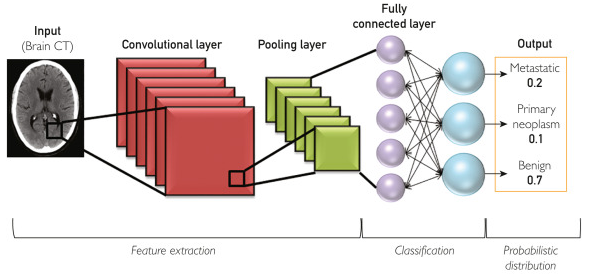
\includegraphics[width=0.8\textwidth]{cnn.png} 
    \caption{Ejemplo de arquitectura de una red neuronal convolucional para clasificación de imágenes. Se observan capas convolucionales (conv) que aplican 
    filtros aprendibles sobre la imagen de entrada, seguidas de capas de pooling que reducen la resolución. Al final, capas totalmente conectadas (FC) procesan 
    las características extraídas para producir la clasificación en alguna de las categorías.} 
    \label{fig:cnn_arch} 
\end{figure}

Las CNN han demostrado ser extremadamente efectivas en visión por computador, logrando reconocer objetos en fotos con gran precisión, segmentar imágenes píxel a píxel, 
detectar rostros, entre muchas otras aplicaciones. En el ámbito de imágenes médicas, han superado enfoques tradicionales al detectar patrones sutiles en radiografías, 
resonancias o microscopías que serían difíciles de modelar manualmente. No obstante, entrenar redes profundas con éxito requiere una gran cantidad de datos
clasificadas de manera manual, siendo de mayor dificultad en el ámbito médico donde la anotación de imágenes es costosa y requiere experiencia especializada.
Cuando el conjunto de datos disponible es limitado, es frecuente recurrir a \textit{aprendizaje por transferencia}, utilizando redes pre-entrenadas en un dominio 
amplio (p. ej., ImageNet) y refinándolas (fine-tuning) sobre la tarea específica, aprovechando características visuales genéricas aprendidas previamente.

Otro aspecto relevante es la \textit{interpretabilidad} de las predicciones de las redes neuronales. Las RNA profundas han sido criticadas como “cajas negras” 
difíciles de entender; sin embargo, se han desarrollado técnicas para visualizar y explicar qué han aprendido. Por ejemplo, en imágenes, métodos como \textit{Grad-CAM} 
(Gradiente-Weighted Class Activation Mapping) permiten resaltar las regiones de la imagen que más contribuyen a una determinada predicción de la red, proporcionando 
pistas sobre qué está “mirando” la CNN al tomar su decisión, pudiendo determinar si la red se basa en características relevantes o si ha aprendido patrones no generalizables
(p. ej. clasificando imagenes por el fondo en lugar del objeto de interés). 

En suma, las redes neuronales (especialmente las convolucionales profundas) constituyen la columna vertebral de muchos sistemas modernos de inteligencia artificial, 
logrando avances sin precedentes en reconocimiento de patrones. En la siguiente sección se explorará cómo estas técnicas de ML y redes neuronales se aplican en el ámbito de la visión por 
computador biomédica, con énfasis en el caso MedMNIST y la clasificación de artrosis en rodillas.

\section{ML aplicado a VC y tareas biomédicas: caso MedMNIST}\label{sec:ml-medical} 
La integración de técnicas de aprendizaje profundo y visión por computadora ha revolucionado el análisis de imágenes biomédicas en 
la última década. Tradicionalmente, la interpretación de imágenes médicas como radiografías, resonancias magnéticas y microscopías 
dependía exclusivamente de la habilidad humana. Sin embargo, en la actualidad, los algoritmos de \textit{deep learning} han igualado 
e incluso superado el desempeño de especialistas en diversas tareas diagnósticas.

Un ejemplo destacado es la empresa Quibim, fundada por el exalumno de la UPV, Ángel Alberich-Bayarri. Quibim ha desarrollado modelos 
basados en inteligencia artificial para la detección del cáncer de próstata en resonancias magnéticas. Su herramienta, QP-Prostate®, 
utiliza algoritmos avanzados para identificar y clasificar lesiones sospechosas en la glándula prostática, mejorando la precisión 
diagnóstica y facilitando la planificación de biopsias dirigidas.

Además, se han entrenado redes neuronales convolucionales para detectar retinopatía diabética en fotografías de retina, cáncer de 
piel en imágenes dermatoscópicas y neumonía en radiografías de tórax, alcanzando niveles de sensibilidad y especificidad 
comparables a los de médicos especialistas. Un metaanálisis realizado por Liu et al. (2019) concluyó que los clasificadores 
basados en aprendizaje profundo presentan, en promedio, un desempeño similar al de profesionales de la salud en la detección de 
enfermedades a partir de imágenes médicas, resaltando el potencial de estas técnicas para apoyar la labor clínica.

En el caso particular de la \textbf{artrosis de rodilla} (u osteoartritis), la radiografía es la técnica más utilizada para evaluar 
la gravedad de la enfermedad. Los radiólogos emplean un criterio estandarizado, la \textit{escala Kellgren-Lawrence (KL)}, que asigna 
un grado de 0 a 4 a la rodilla en función de signos radiográficos de degeneración (osteofitos, estrechamiento del espacio articular, 
esclerosis, deformidad). Sin embargo, la lectura de estas radiografías puede ser subjetiva y presentar variabilidad entre observadores.
Por ello, existe un gran interés en desarrollar sistemas automáticos que clasifiquen el grado KL a partir de la imagen de rayos X de 
la rodilla de forma consistente y reproducible. 

Dado el amplio espectro de modalidades y problemas en imágenes médicas, han surgido iniciativas para facilitar la investigación y 
comparación de algoritmos en múltiples tareas. Un ejemplo es la \textbf{Osteoarthritis Initiative (OAI)}, que ha desarrollado un conjunto 
de datos de radiografías de rodilla con anotaciones de grado Kellgren-Lawrence (KL) el cual se desarrollará mas adelante. 
Otro caso notable es \textbf{MedMNIST}, una colección de conjuntos de datos biomédicos de pequeño tamaño inspirada 
en el famoso MNIST (conjunto de datos de dígitos escritos a mano) pero orientada a imágenes médicas. En su versión más reciente, 
\textit{MedMNIST v2}, recopila 12 conjuntos de datos 2D (imágenes estáticas de 28$\times$28 píxeles) y 6 conjuntos 3D (volúmenes de 
28$\times$28$\times$28 vóxeles), abarcando diversas modalidades y tareas de clasificación biomédica. Por ejemplo, incluye láminas 
histológicas coloreadas (\textit{PathMNIST}, 9 clases de tejidos patológicos), imágenes dermatoscópicas de lunares (\textit{DermaMNIST}, 
clasificación de lesiones cutáneas) y radiografías de tórax (\textit{ChestMNIST}, etiquetas multilabel de hallazgos torácicos), 
hasta estudios de retina OCT (\textit{OCTMNIST}, detección de patologías retinales), entre otros. Cada subconjunto viene preprocesado 
y separado en particiones de entrenamiento, validación y prueba estandarizadas, lo que facilita la aplicación directa de algoritmos 
y la comparación justa entre ellos.

MedMNIST  fue diseñado con varios objetivos clave en mente:
\begin{itemize}
    \item \textbf{Diversidad}: Cubre múltiples modalidades de imagen (radiografías, tomografías, resonancias, ecografías, 
    imágenes microscopias, etc.), distintos tamaños de datos (desde $\sim$100 hasta $>$100,000 imágenes) y tareas de 
    clasificación variadas (binaria, multiclase, multietiqueta e incluso regresión ordinal). Esto permite evaluar la generalización 
    de los algoritmos de aprendizaje automático en distintos escenarios con un solo recurso unificado.
    
    \item \textbf{Estandarización}: Todos los conjuntos están uniformizados a la misma resolución (imágenes pequeñas de $28\times28$ 
    pixeles para 2D, o cubos de $28^3$ para 3D) con formato de datos consistente. Asimismo, se proveen divisiones oficiales en 
    entrenamiento/validación/test para cada dataset. Gracias a esto, los investigadores pueden centrarse en diseñar y probar 
    modelos de \textit{machine learning} sin preocuparse por el preprocesamiento de datos o posibles sesgos en la separación 
    de conjuntos, y los resultados son comparables entre diferentes estudios de forma más directa.
    
    \item \textbf{Ligereza y accesibilidad}:  El reducido tamaño de las imágenes hace que ejecutar experimentos sea computacionalmente 
    liviano, incluso sin hardware especializado. Además, la colección es de libre acceso con licencia abierta (CC BY) y cuenta con una 
    API unificada (disponible vía \texttt{pip install medmnist}) para cargar los datos fácilmente en diversos lenguajes. 
    Esto democratiza la experimentación en análisis de imágenes médicas, permitiendo a estudiantes y grupos con recursos limitados 
    explorar algoritmos de clasificación sobre datos reales de medicina.

    \item \textbf{Benchmark}: MedMNIST sirve tanto para introducir a nuevos usuarios en el campo de la visión médica, al 
    proporcionar casos ya preparados sobre los cuales practicar, como para benchmarking de algoritmos de AutoML y redes 
    neuronales en múltiples tareas livianas. Al enfocarse en imágenes pequeñas, enfatiza más el aspecto algorítmico 
    (diseño del modelo, estrategias de aprendizaje) que el meramente computacional. De hecho, trabajos asociados han 
    evaluado métodos clásicos de deep learning (ResNet, DenseNet, etc.) y herramientas AutoML sobre MedMNIST, generando 
    un punto de referencia inicial de desempeños.
\end{itemize}

En resumen, iniciativas como MedMNIST complementan a los grandes desafíos clínicos (ej. clasificar artrosis en radiografías 
completas) ofreciendo un “laboratorio” controlado para probar métodos de aprendizaje automático en imágenes biomédicas. 
El presente proyecto de TFG se enmarca precisamente en este contexto: la aplicación del aprendizaje automatico 
a la clasificación de artrosis de rodilla, un problema relevante en el campo de la salud musculoesquelética. 
Aprovechando conjuntos de datos como el de OAI \cite{chen2018knee} (con imágenes reales de pacientes) y los avances reportados 
en la literatura, se buscará entrenar un modelo capaz de predecir el estado de la articulación a partir de la radiografía, evaluando su desempeño 
y utilizando técncias de interpretación como \textit{Grad-CAM}. De este modo, se pretende contribuir tanto a la validación de las 
técnicas de aprendizaje profundo en una tarea biomédica específica como a la comprensión de sus alcances y limitaciones en 
un entorno clínico real.


%%%%%%%%%%%%%%%%%%%%%%%%%%%%%%%%%%%%%%%%%%%%%%%%%%%%%%%%%%%%%%%%%%%%%%%%%%%%%%%
%                              CAPÍTULO 3                                     %
%                     DESCRIPCIÓN DEL DATASET OAI                             %
%%%%%%%%%%%%%%%%%%%%%%%%%%%%%%%%%%%%%%%%%%%%%%%%%%%%%%%%%%%%%%%%%%%%%%%%%%%%%%%


\chapter{Dataset OAI y tareas comunes}
\label{chap:corpus}

\section{Introducción}
\label{sec:3_1_introduccion}

La correcta selección y descripción de los conjuntos de datos es fundamental para el desarrollo riguroso de cualquier proyecto de visión por ordenador. En este capítulo, 
presentamos en detalle los dos recursos principales que sustentan este Trabajo de Fin de Grado: el \emph{dataset} OAI y el \emph{dataset} de gatos. Ambos provienen de 
contextos y dominios distintos —medicina radiológica y clasificación zoológica—, lo que nos permite ilustrar la aplicabilidad de las técnicas de aprendizaje profundo en 
entornos diversos y evaluar la robustez de los modelos propuestos.

El \emph{dataset} OAI (\emph{Osteoarthritis Initiative}) constituye un estudio observacional multicéntrico de más de una década de duración, diseñado para captar la 
progresión de la artrosis de rodilla mediante imágenes radiográficas y datos clínicos asociados. Su riqueza en términos de metadatos clínicos, visitas longitudinales 
y variedad de modalidades de imagen lo convierte en un estándar de referencia en la literatura científica sobre artrosis. La explotación de este recurso permite abordar 
tareas de diagnóstico automatizado, prognóstico de la enfermedad y evaluación de biomarcadores, ámbitos que requieren una descripción exhaustiva de las características 
de adquisición, las etiquetas disponibles y los posibles sesgos inherentes al diseño del estudio.

Por su parte, el \emph{dataset} de gatos representa un ejemplo de conjunto de datos de clasificación de imágenes en un dominio completamente distinto. Aunque de menor 
escala, este conjunto aporta diversidad de condiciones de iluminación, posturas y categorías diagnósticas, lo que lo hace idóneo para evaluar la generalización 
de modelos entrenados en contextos médicos a tareas de clasificación más convencionales. Su inclusión en este trabajo busca comparar cómo técnicas similares 
de procesamiento y clasificación responden a datasets con distribuciones y tamaños muy dispares.

Para la anotación de las imágenes radiográficas de rodilla, la escala de severidad convencional es la \textbf{Kellgren-Lawrence (KL)}, un sistema ordinal que clasifica 
la artrosis en cinco grados:
\begin{itemize}
    \item \textbf{Grado 0:} Ausencia de signos radiográficos de artrosis.  
    \item \textbf{Grado 1:} Dudoso; posible pinzamiento mínimo del espacio articular o formación muy incipiente de osteofitos marginales.  
    \item \textbf{Grado 2:} Leve; presencia clara de osteofitos y estrechamiento leve del espacio articular.  
    \item \textbf{Grado 3:} Moderado; múltiples osteofitos de tamaño medio, pinzamiento definido del espacio articular y esclerosis subcondral leve.  
    \item \textbf{Grado 4:} Severo; grandes osteofitos, estrechamiento marcado del espacio articular, esclerosis subcondral significativa y deformidad ósea evidente.  
\end{itemize}
Este enfoque ordinal de graduación sirve de modelo conceptual para definir categorías en ambos conjuntos de datos, facilitando la comparación y el diseño de tareas 
de clasificación tanto en imágenes médicas como en imágenes de gatos.

La sección~\ref{sec:3_2_dataset_oai} describirá con detalle la estructura, particiones y características del \emph{dataset} OAI, enfatizando sus splits, resolución 
de imágenes y distribuciones de clases. Acto seguido, en la sección~\ref{sec:3_3_dataset_gatos} se presentará el \emph{dataset} de gatos, incluyendo su origen, 
tiquetas, número de muestras y proporciones de entrenamiento y validación (70/30). En la sección~\ref{sec:3_4_tareas_comunes} se revisarán las tareas de clasificación 
binaria, multiclase y formulaciones ordinales o de regresión— que se aplican a ambos datasets, junto con consideraciones sobre desbalance de clases, técnicas de 
preprocesamiento y métricas de evaluación. Finalmente, la sección~\ref{sec:3_5_conclusiones} sintetizará las principales observaciones y sentará las bases metodológicas 
para los capítulos posteriores.

Con esta estructura, se busca proporcionar una visión integral de los recursos de datos y de las tareas de clasificación, facilitando la comprensión y reproducibilidad 
de los experimentos realizados.

\section{Dataset OAI}
\label{sec:3_2_dataset_oai}

El \emph{Osteoarthritis Initiative (OAI)} es un estudio observacional, multicéntrico y longitudinal lanzado en 2004 
por los NIH de EE.UU., cuyo objetivo principal ha sido identificar y validar biomarcadores asociados tanto a la 
incidencia como a la progresión de la artrosis de rodilla sintomática. Gracias a su diseño de más de diez años de 
seguimiento, este recurso se ha consolidado como un estándar en la investigación sobre artrosis, proporcionando no 
solo imágenes radiográficas, sino también metadatos clínicos, demográficos y de biospecímenes. Aunque solo se utilizarán
las imágenes radiográficas de rodilla, es importante destacar que el OAI incluye un amplio espectro de datos,

Para facilitar su uso en tareas de aprendizaje automático, se emplea una versión curada de la OAI disponible en 
Mendeley Data y Kaggle. Este recurso procesado consta de 9786 radiografías de rodilla recortadas y preprocesadas, 
con etiquetas de severidad basadas en la escala Kellgren-Lawrence (KL) de 0 a 4, asignadas por radiólogos expertos. 
Los usuarios pueden descargar dos resoluciones estándar (224x224 y 299x299 píxeles) en Mendeley Data, mientras que 
en Kaggle solo se ofrece la versión de 224x224 píxeles, optimizada para arquitecturas CNN como ResNet, VGG, 
EfficientNet e Inception.

La Figura \ref{fig:knee-examples} muestra ejemplos visuales de radiografías correspondientes a cada uno de los grados KL. A pesar de su amplio uso, la escala KL presenta 
limitaciones conocidas, como su subjetividad y variabilidad interobservador, lo que motiva la búsqueda de métodos automáticos y objetivos para la evaluación de la OA 
\cite{chen2019fully}.

\begin{figure}[htbp]
    \centering
    \begin{subfigure}[b]{0.19\textwidth}
        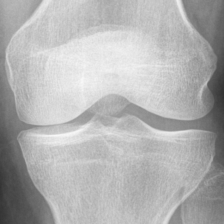
\includegraphics[width=\textwidth]{knee_0.png}
        \caption{KL 0}
        \label{fig:knee0}
    \end{subfigure}
    \hfill
    \begin{subfigure}[b]{0.19\textwidth}
        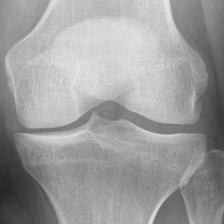
\includegraphics[width=\textwidth]{knee_1.png}
        \caption{KL 1}
        \label{fig:knee1}
    \end{subfigure}
    \hfill
    \begin{subfigure}[b]{0.19\textwidth}
        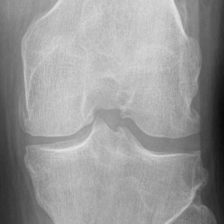
\includegraphics[width=\textwidth]{knee_2.png}
        \caption{KL 2}
        \label{fig:knee2}
    \end{subfigure}
    \hfill
    \begin{subfigure}[b]{0.19\textwidth}
        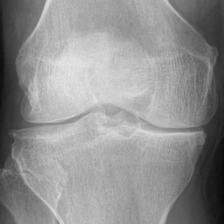
\includegraphics[width=\textwidth]{knee_3.png}
        \caption{KL 3}
        \label{fig:knee3}
    \end{subfigure}
    \hfill
    \begin{subfigure}[b]{0.19\textwidth}
        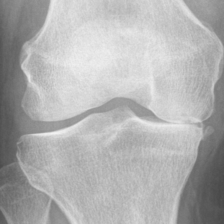
\includegraphics[width=\textwidth]{knee_4.png}
        \caption{KL 4}
        \label{fig:knee4}
    \end{subfigure}
    \caption{Ejemplos de radiografías de rodilla clasificadas según la escala Kellgren \& Lawrence (KL)}
    \label{fig:knee-examples}
\end{figure}

El dataset publicado en Mendeley Data por Chen, estrechamente vinculado a su trabajo posterior sobre clasificación automática de grados KL mediante 
redes neuronales profundas \cite{chen2019fully}, es un ejemplo prominente y fue específicamente organizado para facilitar tareas de detección de la articulación y clasificación 
de la severidad. Las características generales de estas versiones procesadas, que constituyen la base de numerosos estudios posteriores (incluido el presente trabajo), suelen ser 
las siguientes:

\begin{itemize}
    \item \textbf{Imágenes:} El conjunto total incluye \textbf{9\,786 imágenes}, distribuidas en cuatro particiones diferenciadas: \textit{train} (5\,778), \textit{validation} (826), \textit{test} (1\,656) y \textit{auto\_test} (1\,526), como se muestra en la Tabla~\ref{tab:splits}.
    
    \begin{table}[h]
        \centering
        \caption{Distribución de imágenes por partición}
        \label{tab:splits}
        \begin{tabular}{lrr}
            \toprule
            \textbf{Partición} & \textbf{Número de imágenes} & \textbf{Porcentaje} \\
            \midrule
            Entrenamiento (Train) & 5\,778 & 59.04\,\% \\
            Validación (Validation) & 826 & 8.44\,\% \\
            Prueba (Test) & 1\,656 & 16.92\,\% \\
            Autoevaluación (AutoTest) & 1\,526 & 15.59\,\% \\
            \bottomrule
        \end{tabular}
    \end{table}

    \item \textbf{Etiquetas:} Cada imagen está etiquetada con un grado KL (de 0 a 4), siguiendo el criterio de radiólogos expertos de la OAI. Esta información es clave 
    para entrenar modelos supervisados de clasificación.

    \item \textbf{Resolución y preprocesamiento:} En la versión de Mendeley, las imágenes se encuentran disponibles en dos resoluciones estándar: \textbf{224x224} y 
    \textbf{299x299} píxeles, facilitando el uso de arquitecturas preentrenadas como ResNet o EfficientNet. En la versión de Kaggle solo están disponibles en 224x224
    píxeles, lo que la hace más directa para su uso en modelos CNN comunes.

    \item \textbf{Distribución de clases:} La Tabla~\ref{tab:class_distribution} muestra la distribución de clases en el conjunto de entrenamiento. Se observa un claro 
    desbalance hacia las clases más leves de artrosis, lo que debe considerarse en el diseño de los modelos de clasificación.

    \begin{table}[h]
        \centering
        \caption{Distribución de clases en el conjunto de entrenamiento}
        \label{tab:class_distribution}
        \begin{tabular}{lrrrr}
            \toprule
            \textbf{Clase KL} & \textbf{Índice} & \textbf{Imágenes} & \textbf{Porcentaje} \\
            \midrule
            0 (Sin artrosis) & 0 & 2\,286 & 39.56\,\% \\
            1 (Ligera) & 1 & 1\,046 & 18.10\,\% \\
            2 (Leve) & 2 & 1\,516 & 26.24\,\% \\
            3 (Moderada) & 3 & 757 & 13.10\,\% \\
            4 (Severa) & 4 & 173 & 2.99\,\% \\
            \bottomrule
        \end{tabular}
    \end{table}

    \begin{figure}[ht]
        \centering
        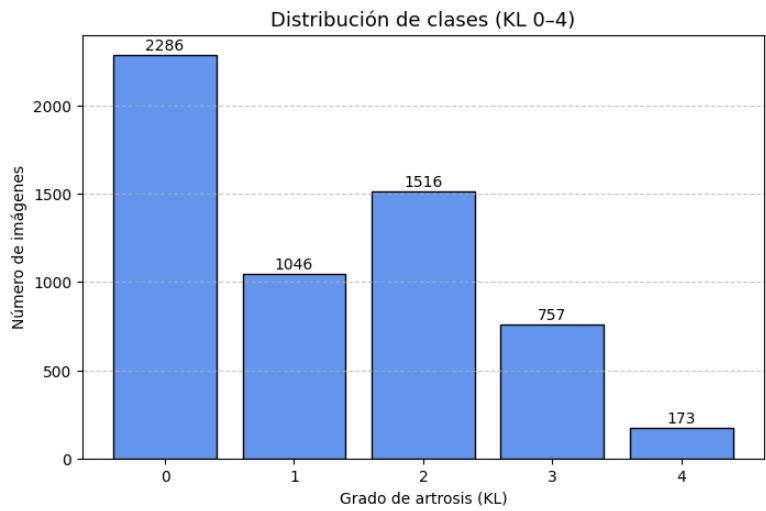
\includegraphics[width=0.7\textwidth]{class_distribution_train.png}
        \caption{Distribución de clases (KL 0 a KL 4) en el conjunto de entrenamiento del dataset OAI. Se observa un desbalance significativo hacia los grados más leves.}
        \label{fig:class_barplot}
    \end{figure}

    Como se observa, el conjunto de entrenamiento presenta un notable desbalance de clases, con predominancia de imágenes etiquetadas con 
    grado 0 (sin artrosis) y grado 2 (leve), y una clara escasez de imágenes con grado 4 (severa). Este desbalance puede inducir a que el modelo 
    favorezca las clases más frecuentes durante el entrenamiento, afectando negativamente su capacidad para detectar los casos más críticos. 

    \item \textbf{Divisiones (Splits):} La existencia de splits predefinidos facilita la reproducibilidad de experimentos y la comparación entre distintos enfoques. 
    Considerando únicamente los subconjuntos \textit{train}, \textit{validation} y \textit{test} —que son los habitualmente utilizados para entrenar y evaluar modelos— 
    se mantiene una proporción aproximada de \textbf{70\,\% entrenamiento}, \textbf{10\,\% validación} y \textbf{20\,\% test}, ampliamente adoptada en la comunidad. 
    El conjunto \textit{auto\_test}, aunque no se utiliza en todos los trabajos, está disponible como recurso adicional que se utiliza en ocasiones para aumentar la cantidad de 
    imagenes en el entrenamiento.
\end{itemize}

\section{Dataset de gatos}
\label{sec:3_3_dataset_gatos}

El \emph{dataset} de gatos es un conjunto de imágenes privadas recopiladas en el marco del Trabajo de Fin de Grado de Bea. 
Aunque de escala reducida en comparación con el \emph{OAI}, aporta un caso de estudio valioso para evaluar la generalización 
de modelos de clasificación entrenados en un dominio tan distinto.

Este conjunto de datos fue obtenido por Bea mediante fotografía controlada de ejemplares felinos, cubriendo diversas 
posturas y condiciones de iluminación. Las imágenes no están disponibles públicamente y su uso queda restringido a fines 
de investigación, bajo autorización expresa de la autora.

El conjunto incluye radiografías de rodillas de gato tanto en vista frontal como lateral, todas ellas anotadas según la 
escala Kellgren-Lawrence (KL). Para mantener la coherencia anatómica y metodológica con el dataset OAI, en este trabajo 
se utilizarán únicamente las proyecciones frontales.

En total se dispone de 83 radiografias de gatos, distribuidas en 5 clases según la severidad de la artrosis. La 
Tabla~\ref{tab:cat_class_distribution} muestra la distribución de clases de todo el dataset.

\begin{table}[h]
    \centering
    \caption{Distribución de clases en el conjunto de entrenamiento}
    \label{tab:cat_class_distribution}
    \begin{tabular}{lrrr}
        \toprule
        \textbf{Clase KL}  & \textbf{Imágenes} & \textbf{Porcentaje} \\
        \midrule
        0 (Sin artrosis)  & 30 & 36,6\,\% \\
        1 (Ligera)        & 21 & 25,6\,\% \\
        2 (Leve)          & 18 & 22,0\,\% \\
        3 (Moderada)      & 11 & 13,4\,\% \\
        4 (Severa)        &  2 &  2,4\,\% \\
        \bottomrule
    \end{tabular}
\end{table}

Este conjunto de imágenes felinas funcionará como un conjunto de validación externo durante el proceso de entrenamiento de 
los modelos basados en el dataset OAI. Su propósito es poner a prueba la capacidad de generalización de los clasificadores 
aprendidos sobre radiografías humanas, aplicándolos a un dominio anatómico distinto pero con la misma tarea de gradación 
de artrosis. Al enfrentar los modelos a variaciones en la morfología articular y en las condiciones de adquisición, 
podremos cuantificar de manera objetiva su robustez frente a cambios de dominio.

El ajuste fino (fine-tuning) se llevará a cabo siguiendo dos vertientes complementarias. En la primera, partiremos de 
arquitecturas preentrenadas en grandes repositorios genéricos (por ejemplo, ImageNet), tal como se realizó en los
experimentos con el dataset OAI. En la segunda, utilizaremos directamente los modelos preentrenados sobre el propio 
dataset OAI, aprovechando sus pesos como punto de partida para un nuevo entrenamiento dirigido al dominio de gatos. 
En ambas estrategias se adoptará un enfoque conservador: las capas iniciales del backbone permanecerán congeladas, 
afinándose únicamente las capas superiores y la cabeza de clasificación. De esta forma, se minimiza el riesgo de 
sobreajuste y se maximiza la transferencia de características útiles a pesar del tamaño reducido del dataset de gatos.

\section{Taras comunes}
\label{sec:common_tasks}

El conjunto de datos de la *Osteoarthritis Initiative* (OAI) ha sido ampliamente empleado en la literatura científica como base para el desarrollo de modelos de aprendizaje
profundo orientados al diagnóstico automatizado de la artrosis de rodilla. Gracias a su riqueza clínica y su volumen de imágenes radiográficas etiquetadas según la escala de
Kellgren-Lawrence (KL), este dataset se ha convertido en una referencia para la validación de nuevas arquitecturas y metodologías dentro del ámbito de la inteligencia 
artificial aplicada a la medicina.

A lo largo del tiempo, diferentes líneas de investigación han coincidido en una serie de tareas recurrentes que abordan distintos enfoques sobre la severidad de la artrosis. 
Estas tareas pueden clasificarse, principalmente, en función de tres criterios:

\begin{itemize}
    \item El tipo de clasificación: binaria (presencia o ausencia de artrosis) o multiclase (grados de KL de 0 a 4).
    \item La metodología de entrenamiento: desde cero (*from scratch*) o mediante *transfer learning* con redes preentrenadas.
    \item La formulación del problema: como clasificación ordinaria o regresión ordinal.
\end{itemize}

Cabe destacar que estas tareas no son excluyentes, y muchas publicaciones recientes exploran combinaciones de estos enfoques. Además, se ha popularizado el uso de técnicas complementarias 
como el ensamblado de modelos (ensembling), el ajuste fino de pesos (fine-tuning) o el uso de funciones de pérdida adaptadas a la naturaleza ordinal del problema.

En el contexto de este Trabajo de Fin de Grado, el foco se centrará exclusivamente en la tarea de clasificación del grado de artrosis, descartando explícitamente la tarea de detección automática de 
la articulación de la rodilla. Se parte de imágenes radiográficas previamente recortadas como se encuentran en los datasets disponibles en Mendeley y Kaggle, donde la articulación ya ha sido
detectada y centrada, pudiendo replicar los experimentos de otros autores y comparar los resultados obtenidos de una manera más directa. 

A modo de ejemplo representativo de las tareas descritas, se presentan a continuación varios estudios recientes que han abordado el problema de clasificación de la artrosis de 
rodilla utilizando el dataset OAI, cada uno desde una perspectiva metodológica distinta. Estos trabajos ilustran bien la diversidad de aproximaciones y motivaciones que existen 
en la literatura científica actual, y permiten contextualizar el enfoque adoptado en este Trabajo de Fin de Grado.

\textbf{Chen et al. (2019)} \cite{chen2019fully} desarrollan un sistema completamente automatizado para la clasificación de la severidad de la 
artrosis de rodilla, combinando detección de la articulación con YOLOv2 y posterior clasificación mediante redes neuronales profundas. 
En el contexto de este TFG, el interés se centra en la segunda fase del pipeline: la predicción del grado de artrosis según la escala de 
Kellgren-Lawrence (KL). Los autores emplean arquitecturas CNN preentrenadas como VGG, ResNet, InceptionV3 y DenseNet, afinadas con una función de 
pérdida personalizada denominada adjustable ordinal loss, diseñada para penalizar más severamente los errores a mayor distancia ordinal. 
Los resultados muestran que esta función mejora el rendimiento frente a la entropía cruzada tradicional, alcanzando una precisión del 70.4\% con 
VGG-19 como mejor modelo. Esta propuesta es destacable por introducir de manera explícita la naturaleza ordinal de las etiquetas KL en el proceso 
de entrenamiento, aspecto esencial para tareas clínicas con niveles de severidad escalonados.

\textbf{Rafique et al. (2024)} \cite{rafique2024knee} proponen un enfoque comprensivo para la clasificación automática de la artrosis 
de rodilla basado en modelos CNN preentrenados y técnicas de inteligencia artificial explicable (XAI). Su metodología evalúa cinco 
arquitecturas (VGG-16, VGG-19, ResNet-50, ResNet-101 y EfficientNetB7) tanto en tareas multiclase (grados KL 0 a 4) como binarias, 
mediante un análisis sistemático de subgrupos (e.g., 0 vs. 1, 0 vs. 2, etc.). Además, aplican Grad-CAM para interpretar las regiones 
de interés utilizadas por los modelos en la toma de decisiones, comparándolas con las zonas anatómicas de evaluación clínica. Sus 
resultados destacan la dificultad de distinguir casos leves (KL1), coincidiendo con otros estudios, mientras que en escenarios binarios 
extremos (e.g., 0 vs. 4), EfficientNetB7 alcanza una precisión del 99.13\%. Esta propuesta resulta especialmente interesante para 
este TFG por su énfasis en interpretabilidad y comparación directa entre estrategias multiclase y binarias, lo cual aporta 
información clave sobre la viabilidad de cada enfoque diagnóstico en entornos reales.

\textbf{Nabil et al. (2024)} \cite{nabil2024automatic} optan por una estrategia simplificada que agrupa las clases KL 0, 1 y 2 bajo la categoría 
“sano”, lo cual responde a la dificultad recurrente en la clasificación precisa del grado KL1. Comparan tres arquitecturas profundas 
—EfficientNetB7, DenseNet169 e InceptionResNetV2— y reportan un rendimiento superior de EfficientNetB7, con una precisión del 93.90\%. 
Su propuesta destaca por una cuidadosa fase de preprocesamiento, uso extensivo de técnicas de aumento de datos y regularización, así 
como una formulación del problema como clasificación en tres niveles (sano, moderado, severo). Pese a su elevado coste computacional, 
EfficientNetB7 se presenta como una solución idónea para entornos clínicos donde la precisión diagnóstica es prioritaria.

\textbf{Fei et al. (2024)} \cite{fei2024diagnosing} plantean un cambio conceptual al abordar la clasificación de la artrosis como un problema 
de regresión continua, en lugar de una clasificación discreta. Utilizando redes neuronales convolucionales, sus modelos generan puntuaciones 
decimales entre 0 y 4 que reflejan con mayor precisión la progresión de la enfermedad. Evalúan cuatro arquitecturas —VGG16, ResNet34, 
DenseNet196 y EfficientNetV2 small— sobre 8260 imágenes del dataset OAI, siendo EfficientNetV2 la más destacada, con una precisión del 71\%, 
AUC de 0.83 y un error absoluto medio (MAE) de 0.42. Este enfoque permite un análisis más granular y continuo del estado articular, abriendo 
la puerta a aplicaciones como el seguimiento longitudinal, la predicción de progresión y el soporte a la decisión clínica.

Cabe destacar que, al igual que la función de pérdida adjustable ordinal loss utilizada por Chen et al. (2019), el uso de una pérdida de tipo 
error cuadrático medio en este estudio refleja la intención de penalizar proporcionalmente según la distancia ordinal entre la predicción y 
la etiqueta real. Aunque desde una perspectiva técnica se trata de una formulación regresiva en lugar de categórica, ambas propuestas comparten 
el objetivo de capturar la estructura ordinal inherente al sistema de gradación de Kellgren-Lawrence, superando así las limitaciones de la entropía 
cruzada convencional.

En la Tabla~\ref{tab:comparative_oai} se presenta una síntesis comparativa de los principales trabajos analizados que han utilizado el dataset OAI. 
Se resumen los modelos empleados, el tipo de tarea formulada y la precisión obtenida en cada caso. Esta 
comparativa permite tener una visión global del panorama actual, así como identificar tendencias metodológicas relevantes para este TFG.

\begin{table}[h]
    \centering
    \caption{Comparativa de tareas y resultados en el dataset OAI}
    \label{tab:comparative_oai}
    \begin{tabular}{lcccccc}
        \toprule
        \textbf{Estudio} & \textbf{KL 0--4} & \textbf{KL 0\raisebox{0.5ex}{*}-3-4} & \textbf{0 vs 1} & \textbf{0 vs 2} & \textbf{0 vs 3} & \textbf{0 vs 4} \\
        \midrule
        Chen et al. (2019)     & 70.4\% & --        & --        & --        & --        & --        \\
        Rafique et al. (2024)  & 58\%   & --        & 78.11\%   & 82.33\%   & 91.53\%   & 99.13\%   \\
        Nabil et al. (2024)    & --     & 94.09\%   & --        & --        & --        & --        \\
        Fei et al. (2024)      & 71\%   & --        & --        & --        & --        & --        \\
        \bottomrule
    \end{tabular}
\end{table}

\vspace{-1ex}
\begin{flushleft}
    \footnotesize\raisebox{0.5ex}{*} 0 agrupa las clases KL 0, 1 y 2 como “sano”, frente a los grados 3 y 4 (“avanzado”).
\end{flushleft}




El análisis de estos trabajos evidencia una creciente tendencia a incorporar la naturaleza ordinal del problema, así como a experimentar 
con formulaciones alternativas como la regresión o el uso de modelos ensamblados. Esta revisión proporciona una base sólida para el diseño 
experimental planteado en los capítulos siguientes, donde se compararán distintos enfoques de clasificación aplicados sobre el dataset OAI, 
considerando también la interpretación de resultados mediante técnicas como Grad-CAM.


%%%%%%%%%%%%%%%%%%%%%%%%%%%%%%%%%%%%%%%%%%%%%%%%%%%%%%%%%%%%%%%%%%%%%%%%%%%%%%%
%                              CAPÍTULO 4                                     %
%                        REDES CONVOLUCIONALES                                %
%%%%%%%%%%%%%%%%%%%%%%%%%%%%%%%%%%%%%%%%%%%%%%%%%%%%%%%%%%%%%%%%%%%%%%%%%%%%%%%

\chapter{Redes Convolucionales}
\label{chap:experiments}


\section{Introducción} 
En este capítulo se presentan los experimentos realizados con el objetivo de evaluar progresivamente distintas 
arquitecturas de redes neuronales en la tarea de clasificación automática del grado de artrosis de rodilla a 
partir de imágenes radiográficas.

Siguiendo una estrategia incremental, se parte del entrenamiento de modelos sencillos, como redes densas y 
pequeñas CNN diseñadas desde cero, para posteriormente avanzar hacia arquitecturas más complejas, finalizando 
con la aplicación de técnicas de \textit{fine-tuning} sobre modelos preentrenados en grandes bases de datos 
generales, como ImageNet.

El planteamiento experimental ha sido diseñado para tratar de replicar y contrastar los resultados obtenidos 
en los principales trabajos revisados en el capítulo anterior, especialmente aquellos que han empleado el 
conjunto de datos derivado del estudio OAI \cite{chen2018knee}. Esta aproximación permite evaluar de forma 
objetiva el impacto de distintos niveles de complejidad arquitectónica en el rendimiento de la tarea, así 
como validar la efectividad del uso de aprendizaje por transferencia en el contexto biomédico.

\section{Modelos}

Con el objetivo de estudiar el efecto de la complejidad arquitectónica en el rendimiento del modelo, se diseñaron cinco 
redes neuronales convolucionales, siguiendo un esquema progresivo. Esta sección describe los tres primeros modelos, 
construidos desde cero, que sirven como base comparativa para los modelos preentrenados presentados posteriormente.

\textbf{CNN simple.}  
Este modelo constituye una línea base minimalista, con una única capa convolucional que permite extraer características 
elementales como bordes y texturas. Presenta un número muy reducido de parámetros, lo que se traduce en tiempos de entrenamiento 
bajos. Su principal utilidad reside en proporcionar una referencia con la que contrastar modelos más complejos.

\begin{itemize}
    \item \texttt{Conv2D(16, kernel\_size=3x3, activation='relu', input\_shape=(224, 224, 3))}
    \item \texttt{MaxPooling2D(pool\_size=2x2)}
    \item \texttt{Flatten()}
    \item \texttt{Dense(num\_classes, activation='softmax' if classification else 'linear')}
\end{itemize}

Aunque su capacidad de representación es limitada, este modelo resulta clave para identificar el impacto marginal 
de cada capa adicional sobre el rendimiento general del sistema.

\textbf{CNN mediana.}  
Este segundo modelo introduce una segunda capa convolucional y una capa densa intermedia, lo que le otorga mayor capacidad 
para extraer y combinar patrones espaciales complejos. El incremento en profundidad y en el número de filtros permite detectar 
características jerárquicas más ricas en las imágenes.

\begin{itemize}
    \item \texttt{Conv2D(32, 3x3, activation='relu', padding='same', input\_shape=(..., ..., 1))}
    \item \texttt{MaxPooling2D(2x2)}
    \item \texttt{Conv2D(64, 3x3, activation='relu', padding='same')}
    \item \texttt{MaxPooling2D(2x2)}
    \item \texttt{Flatten()}
    \item \texttt{Dense(128, activation='relu')}
    \item \texttt{Dense(num\_classes, activation='softmax')}
\end{itemize}

Este modelo representa un equilibrio entre simplicidad y expresividad, ideal para analizar cómo la profundidad de la red y 
la cantidad de filtros afectan a la precisión en la clasificación.

\textbf{CNN profunda.}  
El tercer modelo incrementa notablemente la complejidad mediante la incorporación de tres bloques convolucionales con 
normalización por lotes (\textit{Batch Normalization}) y regularización mediante \textit{Dropout}. Esta arquitectura 
está diseñada para aumentar la capacidad del modelo manteniendo su capacidad de generalización y reduciendo el riesgo 
de sobreajuste.

\begin{itemize}
    \item \textbf{Bloque 1:}
    \begin{itemize}
        \item \texttt{Conv2D(32, 3x3, activation='relu', padding='same', input\_shape=(..., ..., 1))}
        \item \texttt{BatchNormalization()}
        \item \texttt{Conv2D(32, 3x3, activation='relu', padding='same')}
        \item \texttt{BatchNormalization()}
        \item \texttt{MaxPooling2D(2x2)}
        \item \texttt{Dropout(0.25)}
    \end{itemize}
    \item \textbf{Bloque 2:}
    \begin{itemize}
        \item \texttt{Conv2D(64, 3x3, activation='relu', padding='same')}
        \item \texttt{BatchNormalization()}
        \item \texttt{Conv2D(64, 3x3, activation='relu', padding='same')}
        \item \texttt{BatchNormalization()}
        \item \texttt{MaxPooling2D(2x2)}
        \item \texttt{Dropout(0.25)}
    \end{itemize}
    \item \textbf{Bloque 3:}
    \begin{itemize}
        \item \texttt{Conv2D(128, 3x3, activation='relu', padding='same')}
        \item \texttt{BatchNormalization()}
        \item \texttt{Conv2D(128, 3x3, activation='relu', padding='same')}
        \item \texttt{BatchNormalization()}
        \item \texttt{MaxPooling2D(2x2)}
        \item \texttt{Dropout(0.4)}
    \end{itemize}
    \item \textbf{Clasificación:}
    \begin{itemize}
        \item \texttt{Flatten()}
        \item \texttt{Dense(256, activation='relu')}
        \item \texttt{BatchNormalization()}
        \item \texttt{Dropout(0.5)}
        \item \texttt{Dense(num\_classes, activation='softmax')}
    \end{itemize}
\end{itemize}

Gracias a esta estructura jerárquica y regularizada, el modelo es capaz de aprender representaciones 
más abstractas y complejas, lo que resulta especialmente útil en el análisis de imágenes médicas donde 
los detalles sutiles pueden ser determinantes para la clasificación. El uso de normalización y regularización 
permite entrenar arquitecturas profundas sin incurrir en problemas de inestabilidad numérica o sobreajuste excesivo.


Modelo 4: \textbf{EfficientNetB0} 

Modelo 5: \textbf{resnetAlfons} o \textbf{ResNet50}

\section{Experimentos}

El diseño experimental de este trabajo se ha estructurado para evaluar el impacto de la complejidad arquitectónica y la transferencia de conocimiento 
en la tarea de clasificación de artrosis de rodilla. Para ello, se han entrenado y comparado cinco modelos representativos bajo condiciones homogéneas.

\textbf{Comparación de modelos con distinta complejidad.}
Se han considerado cinco arquitecturas con creciente capacidad de representación: tres modelos construidos desde cero (CNN simple, CNN pequeña y CNN profunda) 
y dos modelos preentrenados (EfficientNetB0 y ResNet50), ajustados mediante \textit{transfer learning}. Esta selección permite analizar la relación entre la 
expresividad del modelo, el coste computacional y la capacidad de generalización, tanto dentro del dominio (OAI) como fuera de él (radiografías de gatos).

\textbf{Configuración común de entrenamiento.}
Todos los modelos se han entrenado con los mismos hiperparámetros base: optimizador Adam, tasa de aprendizaje inicial de $10^{-3}$, función de pérdida
\texttt{CrossEntropyLoss}, tamaño de lote de 32 y un máximo de 50 épocas. Se ha aplicado \textit{early stopping} con paciencia de 10 épocas sin mejora 
en el conjunto de validación, y un \textit{scheduler} de tasa de aprendizaje con factor de reducción de 0.5 tras 5 épocas sin mejora.

En el caso de los modelos preentrenados, se han evaluado dos variantes: (i) congelando inicialmente el \textit{backbone} y afinando solo las capas finales; 
y (ii) realizando un ajuste fino completo. En ambos casos se ha empezado con una tasa de aprendizaje más baja ($10^{-4}$) debido a la mayor complejidad de
los modelos y la posibilidad de sobreajuste. Esta estrategia busca maximizar la transferencia de conocimiento y minimizar el riesgo de inestabilidad durante el
entrenamiento.

\textbf{División de datos y normalización.}
Todos los entrenamientos se han realizado utilizando las particiones oficiales del dataset OAI (\texttt{train}, \texttt{validation}, \texttt{test}), 
manteniendo su integridad para asegurar la replicabilidad. Las imágenes fueron redimensionadas a 224x224 píxeles y normalizadas para su compatibilidad 
con modelos preentrenados.

\textbf{Evaluación en dominio externo: dataset felino.}
Como medida de validación externa, se ha utilizado un conjunto adicional de imágenes de radiografías de gatos. Durante el entrenamiento, este conjunto 
se ha empleado como evaluación secundaria (no influenciada por el \textit{early stopping} ni el \textit{scheduler}) para estimar la capacidad de generalización 
de los modelos a un dominio visual distinto pero clínicamente análogo. Para cada modelo se ha conservado la mejor versión según la validación humana 
y otra según el rendimiento en gatos.

\textbf{Métricas de evaluación.}
El rendimiento de cada arquitectura se ha evaluado mediante varias métricas: precisión global (\textit{accuracy}), F1-score macro, matriz de confusión 
y error absoluto medio (MAE) para formulaciones ordinales. Estas métricas se han aplicado tanto al conjunto de test del dataset OAI como al conjunto 
felino, permitiendo un análisis cruzado entre dominios. Para la comparación de modelos se ha utilizado la precisión global como métrica principal.

\textbf{Técnicas de regularización y aumento de datos.}
Los modelos diseñados desde cero incluyen mecanismos de regularización como \texttt{Dropout} y \texttt{BatchNormalization}, cruciales para mejorar la 
estabilidad del entrenamiento y mitigar el sobreajuste. Además, se ha implementado \textit{data augmentation} en tiempo real: rotaciones aleatorias, 
reflejos verticales y horizontales, y variaciones de brillo y contraste. Estas transformaciones buscan enriquecer la variabilidad del conjunto de entrenamiento 
y mejorar la robustez del modelo.


\textbf{Resultados simple CNN:}

\begin{table}[h]
    \centering
    \caption{Resultados Simple CNN en clasificación y regresión}
    \label{tab:simple_cnn_results_improved}
    \begin{tabular}{@{} l l l c c c c c c @{}} 
      \toprule
      \textbf{Dataset} & \textbf{Tarea} & \textbf{Métrica} 
        & \multicolumn{6}{c}{\textbf{Particiones}} \\
      \cmidrule(lr){4-9}
      & & & 0--4 & 0-3-4 & 0 vs 1 & 0 vs 2 & 0 vs 3 & 0 vs 4 \\
      \midrule
      % Clasificación OAI
      \multirow{2}{*}{OAI}
        & Clasif. & Accuracy   & 42\%   & 85.35\%   & 68.19\% &  65.37\%   &  80.88\%   &  97.18\%   \\
        & Clasif. & F1-score    & 30\%  & 80.35\%  & 55.29\%  &  62.84\%   &  77.98\%   &  97.02\%   \\
      \addlinespace
      % Clasificación Gatos
      \multirow{2}{*}{Gatos}
        & Clasif. & Accuracy   & 25\%   & 83.8\%  & 57.69\% &  65\%     &  69.70\%   &  95.83\%   \\
        & Clasif. & F1-score    & 11\%  & 77\%    & 57.88\% &  63.66\%  &  63.37\%   &  95.19\%   \\
      \midrule
      % Regresión OAI
      \multirow{3}{*}{OAI}
        & Regr.   & Accuracy   & 34.87\%   & 84.38\% &  --      &  --   &  --   &  --   \\
        & Regr.   & F1-score    & 34.65\%  & 78.16\%  &  --      &  --   &  --   &  --   \\
        & Regr.   & MAE         & 0.897  & 0.291  &  --      &  --   &  --   &  --   \\
      \addlinespace
      % Regresión Gatos
      \multirow{3}{*}{Gatos}
        & Regr.   & Accuracy   & 31\%   & 84.34\%  &  --    &  --   &  --   &  --   \\
        & Regr.   & F1-score    & 23\%  & 77.17\%  &  --    &  --   &  --   &  --   \\
        & Regr.   & MAE         & 1.014  & 0.181   &  --    &  --   &  --   &  --   \\
      \bottomrule
    \end{tabular}
\end{table}
  


\textbf{Resultados CNN mediana:}

\begin{table}[h]
    \centering
    \caption{Resultados CNN mediana en clasificación y regresión}
    \label{tab:cnn_mediana_results}
    \begin{tabular}{@{} l l l c c c c c c @{}} 
      \toprule
      \textbf{Dataset} & \textbf{Tarea} & \textbf{Métrica} 
        & \multicolumn{6}{c}{\textbf{Particiones}} \\
      \cmidrule(lr){4-9}
      & & & 0--4 & 0-3-4 & 0 vs 1 & 0 vs 2 & 0 vs 3 & 0 vs 4 \\
      \midrule
      % Clasificación OAI
      \multirow{2}{*}{OAI}
        & Clasif. & Accuracy   & 46.85\% & 85.35\% & 68.19\% & 62.41\% & 84.10\% & 97.46\% \\
        & Clasif. & F1-score   & 39.71\% & 80.35\% & 55.29\% & 54.41\% & 82.16\% & 97.35\% \\
      \addlinespace
      % Clasificación Gatos
      \multirow{2}{*}{Gatos}
        & Clasif. & Accuracy   & 28.92\% & 85.54\% & 42.31\% & 55.00\% & 72.73\% & 100\% \\
        & Clasif. & F1-score   & 18.89\% & 79.29\% & 25.16\% & 39.03\% & 65.60\% & 100\% \\
      \midrule
      % Regresión OAI
      \multirow{3}{*}{OAI}
        & Regr.   & Accuracy   & 34.87\% & 84.02\% & -- & -- & -- & -- \\
        & Regr.   & F1-score   & 34.65\% & 82.71\% & -- & -- & -- & -- \\
        & Regr.   & MAE        & 0.771 & 0.237 & -- & -- & -- & -- \\
      \addlinespace
      % Regresión Gatos
      \multirow{3}{*}{Gatos}
        & Regr.   & Accuracy   & 38.55\% & 84.34\% & -- & -- & -- & -- \\
        & Regr.   & F1-score   & 22.44\% & 77.17\% & -- & -- & -- & -- \\
        & Regr.   & MAE        & 0.9713 & 0.211 & -- & -- & -- & -- \\
      \bottomrule
    \end{tabular}
\end{table}

\textbf{Resultados CNN grende:}
 
\begin{table}[h]
    \centering
    \caption{Resultados CNN grende en clasificación y regresión}
    \label{tab:cnn_grande_results}
    \begin{tabular}{@{} l l l c c c c c c @{}} 
      \toprule
      \textbf{Dataset} & \textbf{Tarea} & \textbf{Métrica} 
        & \multicolumn{6}{c}{\textbf{Particiones}} \\
      \cmidrule(lr){4-9}
      & & & 0--4 & 0-3-4 & 0 vs 1 & 0 vs 2 & 0 vs 3 & 0 vs 4 \\
      \midrule
      % Clasificación OAI
      \multirow{2}{*}{OAI}
        & Clasif. & Accuracy   & 58.47\% & 89.35\% & 68.40\% & 74.26\% & 86.64\% & 99.72\% \\
        & Clasif. & F1-score   & 52.03\% & 88.50\% & 55.78\% & 72.51\% & 86.14\% & 99.72\% \\
      \addlinespace
      % Clasificación Gatos
      \multirow{2}{*}{Gatos}
        & Clasif. & Accuracy   & 34.94\% & 85.54\% & 53.85\% & 62.50\% & 66.67\% & 95.83\% \\
        & Clasif. & F1-score   & 18.89\% & 79.29\% & 52.98\% & 61.99\% & 53.33\% & 95.19\% \\
      \midrule
      % Regresión OAI
      \multirow{3}{*}{OAI}
        & Regr.   & Accuracy   & 43.95\% & 84.34\% & -- & -- & -- & -- \\
        & Regr.   & F1-score   & 46.22\% & 77.17\% & -- & -- & -- & -- \\
        & Regr.   & MAE        & 0.651 & 0.171 & -- & -- & -- & -- \\
      \addlinespace
      % Regresión Gatos
      \multirow{3}{*}{Gatos}
        & Regr.   & Accuracy   & 39.76\% & -- & -- & -- & -- & -- \\
        & Regr.   & F1-score   & 29.65\% & -- & -- & -- & -- & -- \\
        & Regr.   & MAE        & 0.893 & -- & -- & -- & -- & -- \\
      \bottomrule
    \end{tabular}
\end{table}

\textbf{Resultados EfficientNetB0:}
\begin{table}[h]
    \centering
    \caption{Resultados EfficientNetB0 en clasificación y regresión}
    \label{tab:cnn_grande_results}
    \begin{tabular}{@{} l l l c c c c c c @{}} 
      \toprule
      \textbf{Dataset} & \textbf{Tarea} & \textbf{Métrica} 
        & \multicolumn{6}{c}{\textbf{Particiones}} \\
      \cmidrule(lr){4-9}
      & & & 0--4 & 0-3-4 & 0 vs 1 & 0 vs 2 & 0 vs 3 & 0 vs 4 \\
      \midrule
      \multirow{2}{*}{OAI}
        & Clasif. & Accuracy   & 68.64\% & 94.07\% & 74.01\% & 87.22\% & 97.70\% & ?? \\
        & Clasif. & F1-score   & 64.82\% & 93.84\% & 71.78\% & 87.77\% & 97.67\% & ?? \\
      \addlinespace
      \multirow{2}{*}{Gatos}
        & Clasif. & Accuracy   & 25.30\% & 84.34\% & 55.77\% & 60\% & 66.67\% &  \\
        & Clasif. & F1-score   & 10.91\% & 77.17\% & 46.73\% & 60\% & 53.33\% &  \\
      \midrule
      \multirow{3}{*}{OAI}
        & Regr.   & Accuracy   & 65.13\% & 93.83\% & -- & -- & -- & -- \\
        & Regr.   & F1-score   & 65.84\% & 93.67\% & -- & -- & -- & -- \\
        & Regr.   & MAE        & 0.463   & 0.102   & -- & -- & -- & -- \\
      \addlinespace
      \multirow{3}{*}{Gatos}
        & Regr.   & Accuracy   & 36.14\% & 85.54\% & -- & -- & -- & -- \\
        & Regr.   & F1-score   & 19.19\% & 79.89\% & -- & -- & -- & -- \\
        & Regr.   & MAE        & 0.8498 & 0.2120 & -- & -- & -- & -- \\
      \bottomrule
    \end{tabular}
\end{table}



  
\section{Conclusiones}

%%%%%%%%%%%%%%%%%%%%%%%%%%%%%%%%%%%%%%%%%%%%%%%%%%%%%%%%%%%%%%%%%%%%%%%%%%%%%%%
%                              CAPÍTULO 5                                     %
%                             TRANSFORMERS                                    %
%%%%%%%%%%%%%%%%%%%%%%%%%%%%%%%%%%%%%%%%%%%%%%%%%%%%%%%%%%%%%%%%%%%%%%%%%%%%%%%

\chapter{Transformers}
\label{chap:transformers}

\section{Introducción}
En este capítulo se presenta el uso de modelos Transformers en la clasificación automática del grado de artrosis de rodilla a partir de imágenes radiográficas. Los Transformers, 
introducidos inicialmente para tareas de procesamiento de lenguaje natural, han demostrado un rendimiento sobresaliente en visión por computadora gracias a su capacidad para capturar 
relaciones globales en las imágenes mediante mecanismos de atención.

El planteamiento experimental sigue una estrategia progresiva, comenzando con modelos Transformer básicos como Vision Transformer (ViT) y avanzando hacia arquitecturas más sofisticadas 
como Swin Transformer y variantes híbridas que combinan bloques convolucionales y transformadores. Este enfoque permite analizar cómo el uso de atención global y local impacta en el 
rendimiento de la clasificación.

\section{Modelos}
Para evaluar el desempeño de los Transformers en esta tarea, se han seleccionado tres arquitecturas representativas:

\textbf{Vision Transformer (ViT).}
Un modelo Transformer puro que divide las imágenes en parches y aplica atención auto-regresiva para capturar relaciones globales entre estos. Su simplicidad y 
capacidad de escalabilidad lo convierten en un buen punto de partida.

\begin{itemize}
\item 	\texttt{Patch Embedding (16x16)}
\item 	\texttt{Multi-Head Self-Attention (12 heads)}
\item 	\texttt{MLP Head (hidden\_dim=3072)}
\item 	\texttt{Classification Head (num\_classes)}
\end{itemize}

\textbf{Swin Transformer.}
Este modelo introduce ventanas deslizantes para limitar el alcance de la atención, mejorando la eficiencia en imágenes de alta resolución sin perder contexto global.

\begin{itemize}
\item 	\texttt{Patch Embedding (4x4)}
\item 	\texttt{Swin Block (Window Size=7)}
\item 	\texttt{Shifted Window Mechanism}
\item 	\texttt{MLP Head}
\item 	\texttt{Classification Head}
\end{itemize}

\textbf{Hybrid Transformer (ResNet + Transformer).}
Un modelo híbrido que combina un backbone convolucional (ResNet) para extracción de características locales con un bloque Transformer para capturar relaciones globales.

\begin{itemize}
\item 	\texttt{Backbone: ResNet50}
\item 	\texttt{Transformer Encoder (Multi-Head Self-Attention)}
\item 	\texttt{Classification Head}
\end{itemize}

\section{Experimentos}
Los experimentos se han diseñado para evaluar el rendimiento de los modelos Transformer bajo condiciones homogéneas, utilizando las mismas configuraciones de entrenamiento que en el capítulo anterior:

\begin{itemize}
\item Optimizer: Adam
\item Learning Rate: $10^{-4}$
\item Loss Function: CrossEntropyLoss
\item Batch Size: 32
\item Early Stopping: 10 epochs
\item Learning Rate Scheduler: Factor 0.5 after 5 epochs
\end{itemize}

Se han entrenado los modelos en el conjunto de datos OAI, y se ha realizado una evaluación cruzada utilizando un conjunto externo de imágenes de radiografías de gatos, 
para analizar su capacidad de generalización.

\textbf{Métricas de evaluación.}
Las métricas utilizadas para comparar el rendimiento de los modelos son:

\begin{itemize}
\item Precisión global (Accuracy)
\item F1-Score macro
\item Matriz de confusión
\item MAE (Mean Absolute Error)
\end{itemize}

\textbf{Aumento de datos y regularización.}
Se ha aplicado aumento de datos en tiempo real, incluyendo rotaciones aleatorias, reflejos y variaciones de brillo y contraste. Además, se ha utilizado Dropout y 
Normalización por Lotes para mejorar la generalización.

\textbf{Evaluación en dominio externo.}
Se ha evaluado el rendimiento de los modelos en un conjunto adicional de imágenes de radiografías de gatos, replicando las condiciones de evaluación establecidas 
para los modelos convolucionales.


%%%%%%%%%%%%%%%%%%%%%%%%%%%%%%%%%%%%%%%%%%%%%%%%%%%%%%%%%%%%%%%%%%%%%%%%%%%%%%%
%                              CAPÍTULO 5                                     %
%                     TERCERA CONTRIBUCIÓN (OBJETIVO 3)                       %
%%%%%%%%%%%%%%%%%%%%%%%%%%%%%%%%%%%%%%%%%%%%%%%%%%%%%%%%%%%%%%%%%%%%%%%%%%%%%%%
\chapter{Fine-tuning para radiografías de gatos}
\label{chap:finetuning_cats}

\section{Introducción}
\label{sec:cat_intro}


\chapter{Conclusiones}  % ~5 páginas

\section{Resumen del trabajo realizado} % 6.1
% Repasa y sintetiza las secciones principales

\section{Objetivos alcanzados}         % 6.2
% Verifica si se cumplieron los objetivos planteados

\section{Trabajo futuro}               % 6.3
% Explica las posibles extensiones o mejoras

%%%%%%%%%%%%%%%%%%%%%%%%%%%%%%%%%%%%%%%%%%%%%%%%%%%%%%%%%%%%%%%%%%%%%%%%%%%%%%%
%                              BIBLIOGRAFÍA                                   %
%%%%%%%%%%%%%%%%%%%%%%%%%%%%%%%%%%%%%%%%%%%%%%%%%%%%%%%%%%%%%%%%%%%%%%%%%%%%%%%

\printbibliography 
\cleardoublepage

%%%%%%%%%%%%%%%%%%%%%%%%%%%%%%%%%%%%%%%%%%%%%%%%%%%%%%%%%%%%%%%%%%%%%%%%%%%%%%%
%                           APÉNDICES (OPCIONALES)                            %
%%%%%%%%%%%%%%%%%%%%%%%%%%%%%%%%%%%%%%%%%%%%%%%%%%%%%%%%%%%%%%%%%%%%%%%%%%%%%%%

\APPENDIX

\chapter{Configuración del sistema}
% ...

\chapter{Otro apéndice}
% ...

\end{document}
